%
% File: chap04.tex
% Author: Abhushan Sahu
% Description: Introduction chapter where the stuff goes on.
%
\let\textcircled=\pgftextcircled
\chapter{System Design}
\label{chap:intro}

\initial{S}ystems design is the process of defining the architecture, components, modules, interfaces, and data for a system to satisfy specified requirements. Systems design could be seen as the application of systems theory to product development. There is some overlap with the disciplines of systems analysis, systems architecture and systems engineering



%=======


\section{Flowcharts}
\label{sec:sec01}
A flowchart is a type of diagram that represents an algorithm, work-flow or process, showing the steps as boxes of various kinds, and their order by connecting them with arrows. This diagrammatic representation illustrates a solution model to a given problem. Flowcharts are used in analyzing, designing, documenting or managing a process or program in various fields.\\
 Like other types of diagrams, they help visualize what is going on and thereby help understand a process, and perhaps also find flaws, bottlenecks, and other less-obvious features within it. \\
Considering the above lines to be true, here a flowchart of the application system (almost complete). 


\begin{figure}[h]
	\centering
	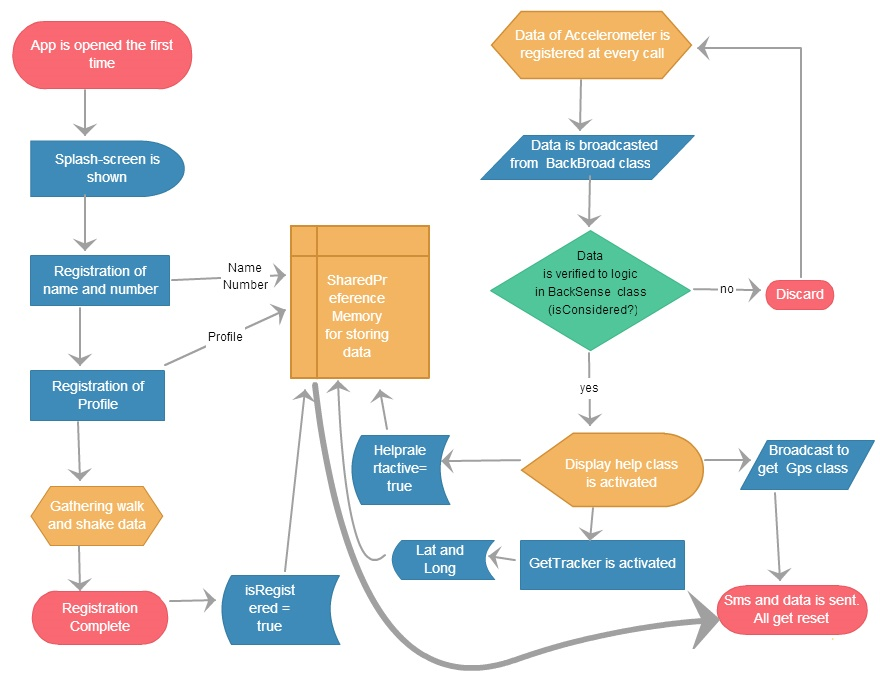
\includegraphics[height=0.6\textheight]{fig01/d_flowc}
	\mycaption[Flow-chart of System.]{Flow-chart of System.}
	\label{fig:RHP01}

\end{figure}

\newpage
\section{Database Design}
\label{sec:sec02}

No database has been used in this system.\\
Though in server, we use one, which has the following structure: \\
u197875796\_extra : is the database name.\\
helpr : while this is the table name.\\


\begin{center}
\begin{tabular}{ c c c c c }
  
Column-name & Type & Length & Attribute & Default\\
sl & int & 11 & Primary-key & Auto-increment\\
name & varchar & 20\\
sos & varchar & 10\\
lat & varchar & 20\\
lon & varchar & 20\\
an\_da & varchar & 30 \\
sy\_da & timestamp & & & Current time\\
\end{tabular}
\end{center}
\vspace{0.6cm}
Here, these terms are:
\begin{description}
\item[$\cdot$ c1] sl : serial number or primary key.
\item[$\cdot$ c2] name : name of user.
\item[$\cdot$ c3] sos : user's sos number.
\item[$\cdot$ c4] lat : current latitude of user on map.
\item[$\cdot$ c5] lon : current longitude of user on map.
\item[$\cdot$ c6] an\_da : system time of user's device.
\item[$\cdot$ c7] sy\_da : time at which the database entry is created.
\end{description}


%\section{Data Flow Diagram}
%\label{sec:sec03}

